 



\section{Experiments} \label{exp}


\subsection{Research Questions}
\label{sec:exp_rqs}

We evaluate CrossLeak by answering the following research questions.

\textbf{RQ1: How effectively does CrossLeak infer deleted labels and deletion-sensitive features compared with state-of-the-art unlearning privacy leakage methods?}

\textbf{RQ2: What are the contributions of CrossLeak's key components, including the CrossCoder and different label inference heads, and how do parameter choices and evaluation metrics affect its performance?}

\textbf{RQ3: How well does CrossLeak generalize to other unlearning scenarios, such as backdoor-trigger recovery and label inference under different unlearning methods?}





\subsection{Experimental Setting}



\noindent
\textbf{Datasets.}
We conduct experiments on three widely used image classification datasets: CIFAR-10 \citep{krizhevsky2009learning}, CIFAR-100 \citep{krizhevsky2009learning}, and Tiny-ImageNet \citep{le2015tiny}. These datasets cover different label spaces and visual complexities, from 10-class object recognition to fine-grained 100-class classification and 200-class large-scale recognition. 



\noindent
\textbf{Models.}
We select the CNN, ViT and ResNet-18 model architectures in our experiments, where as the main model architecture is ResNet-18 on CIFAR10, CIFAR100, and TinyImageNet. We train each original model for 40 epochs with a learning rate of $\eta=0.0001$ and a mini-batch size of 200. All algorithms are implemented using Pytorch and are conducted on NVIDIA A100 GPUs. 



\noindent
\textbf{Federated Unlearning Methods.}
We evaluate CrossLeak under both exact and approximate unlearning settings. For exact unlearning, we use federated retraining on the retained data as the gold-standard baseline, which removes the direct training contribution of deleted samples by training from scratch without them. For approximate unlearning, we consider representative federated unlearning methods, including FedU~\citep{wang2024fedu} and Hessian-based federated unlearning (Hessian-FU/HBFU)~\citep{liu2022right}. This selection allows us to examine whether privacy leakage arises only from approximate update procedures or also remains observable after stronger retraining-based removal. 

%We additionally report the utility of the unlearned model and membership inference attack (MIA) behavior to ensure that leakage is not measured in isolation from standard unlearning quality indicators.


\noindent
\textbf{Attack Baselines.}
We compare CrossLeak with the latest unlearning-targeted model inversion attack~\citep{hu2024learn,wang2025label, zhou2026model}. Since prior attacks mainly reconstruct or infer deleted samples from model gradients and outputs, we adapt their outputs to the same evaluation target by mapping recovered evidence to deleted labels and deletion-sensitive visual concepts when applicable. For unlearning labels inference, we include the \citep{hu2024learn} with confidence-drop and ULIA \citep{wang2025label}. For sensitive feature inference, we just evaluate the CrossLeak because our setting is much more practical, only having the models after aggregation. By contrast, existing studies \citep{hu2024learn, zhou2026model} highly relied on the gradients for single unlearning samples, which are inaccessible in privacy-preserving federated unlearning with secure aggregation.


 
\noindent
\textbf{Metrics.}
For deleted-label inference, we report label inference overlap, i.e., the fraction of true deleted labels that appear in the predicted deleted-label set. In our class-range experiments, the attacker does not know the number of deleted classes, but we report the top-k number of predicted labels, which is matched to the number of deleted target classes. For deletion-sensitive feature inference, we report the fraction of recovered features that overlap with erased-data-sensitive features, denoted as feature-overlap@$k$, the before-exclusive strength ratio measuring how much recovered feature mass is associated with pre-unlearning information, and target-label feature coverage. For semantic interpretability, we also evaluate CLIP-based concept recovery using concept coverage.

%\noindent
%\textbf{Implementation Details.}
%CrossLeak trains a sparse CrossCoder on paired pre- and post-unlearning representations collected from a public probe set. Unless otherwise specified, the probe set is disjoint from the deleted training samples and the attacker does not access the deleted data during inference; deleted labels are used only for evaluation. We report mean and variance over multiple random seeds. All algorithms are implemented in PyTorch and run on NVIDIA A100 GPUs.





\begin{figure*}[t]
	\centering
	\hspace{-2mm}
	\subfloat{  \rotatebox{90}{ \hspace{10mm}	\footnotesize{On CIFAR10} }
		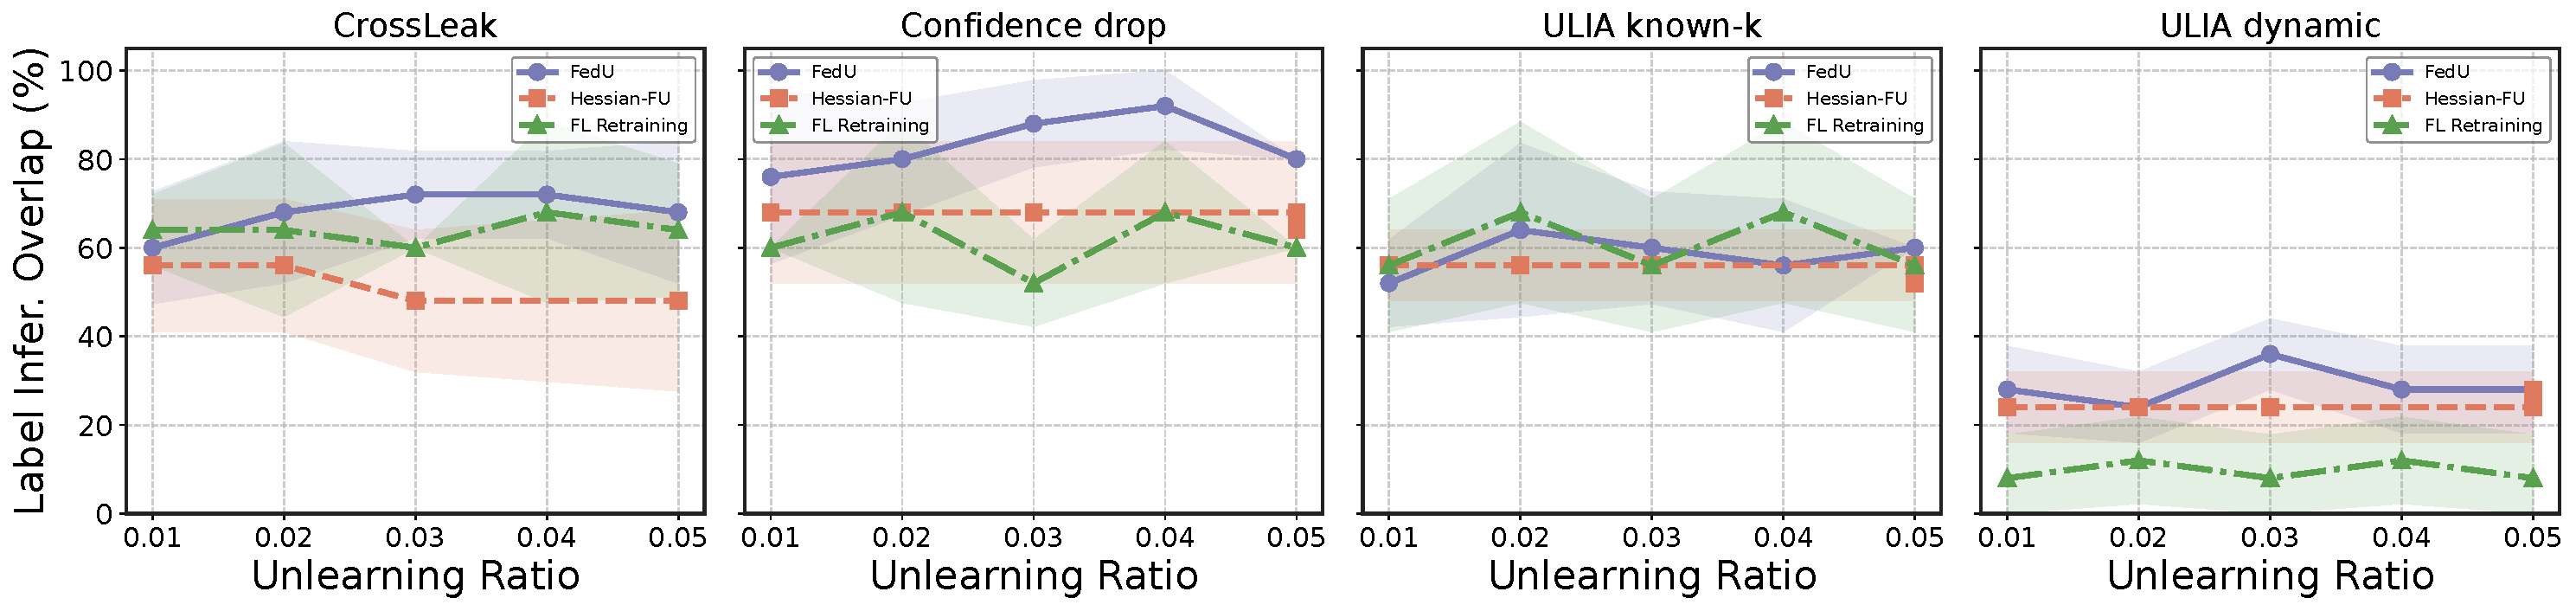
\includegraphics[scale=0.32]{../Exp_results/On_CIFAR10/figures_attacks_ratio/CIFAR10_Attacks_unl_ratio_label_inference_overlap}
	} \\
	\hspace{-2mm}
	\subfloat{  \rotatebox{90}{ \hspace{10mm}	\footnotesize{On CIFAR100} }
		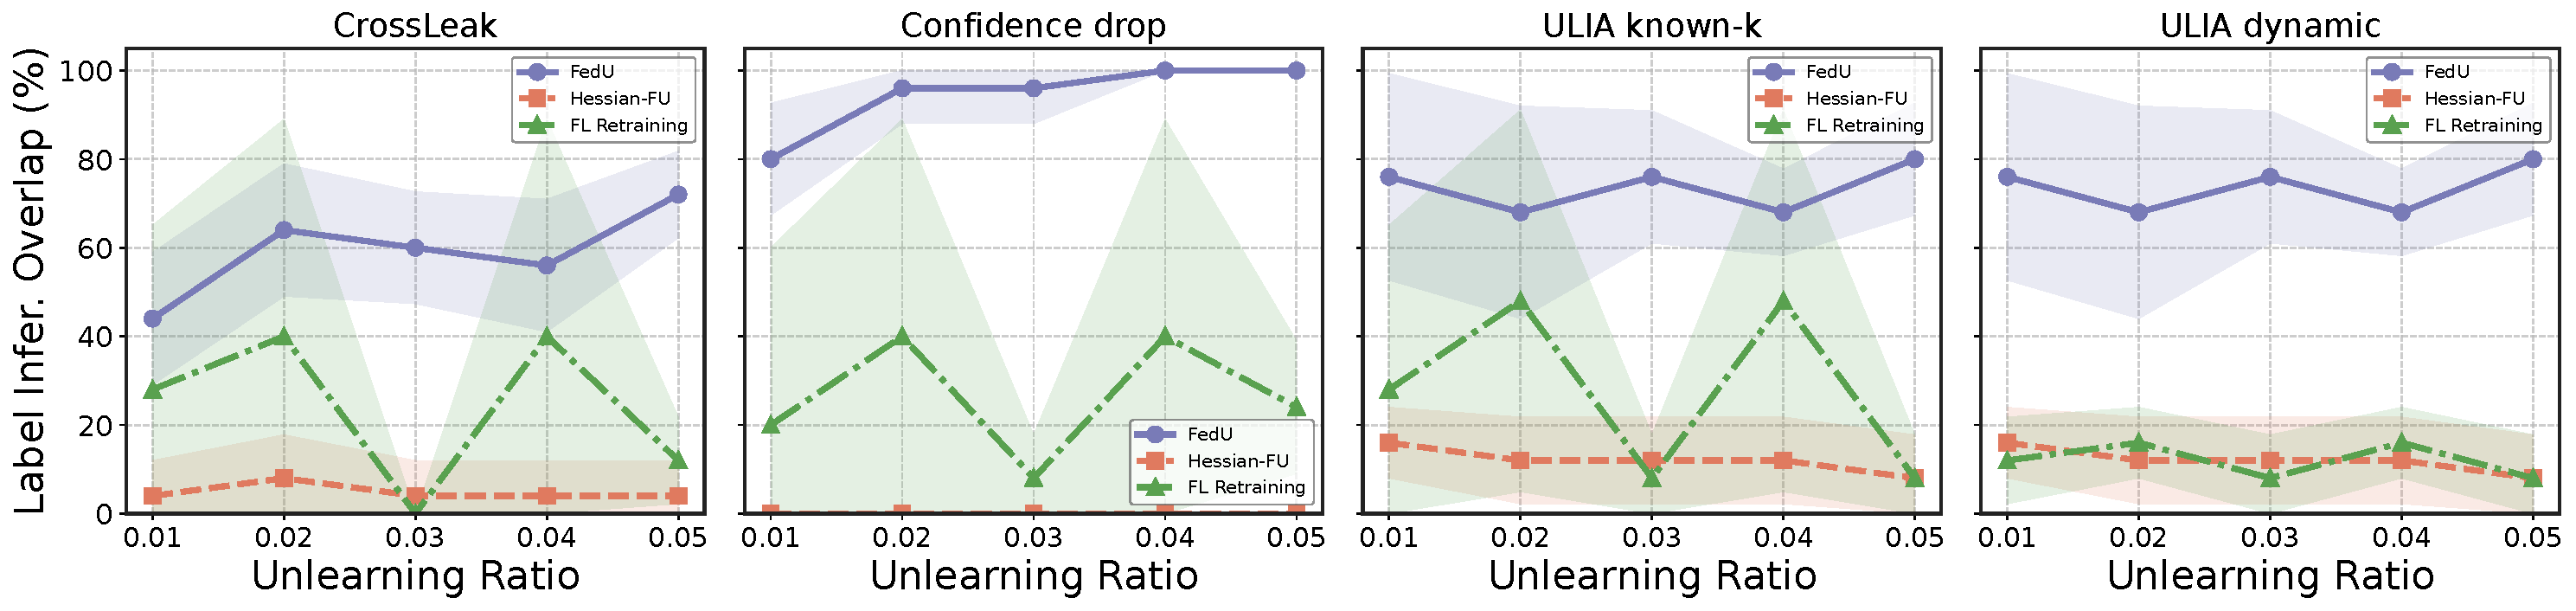
\includegraphics[scale=0.32]{../Exp_results/On_CIFAR100/figures_attacks_ratio/CIFAR100_Attacks_unl_ratio_label_inference_overlap}
	}
	\caption{Label Inference of Different Unlearning Ratio}
	\label{fig:label_inf_ratio}
\end{figure*}


\subsection{RQ1: Privacy Leakage Effectiveness}


\noindent
\textbf{Overall Setup.} In the experiments, for each dataset and each unlearning method, we first train an original federated model $f_{\theta_o}$ on the full training set. We then construct an unlearning request by deleting samples associated with a target label set $Y_u$. To evaluate the impact of deletion scale, we vary the deletion ratio from $1\%$ to $5\%$ of the training data. To evaluate the impact of deletion diversity, we also vary the deleted class range, where $|Y_u|$ controls the number of target labels involved in the unlearning request. We use FedU, Hessian-FU, and exact federated retraining to obtain the post-unlearning model $f_{\theta_u}$, and repeat the experiment over 5 random seeds.

%For each pair $(f_{\theta_o},f_{\theta_u})$, CrossLeak uses a public probe set that is disjoint from the deleted samples. The attacker does not observe the deleted data or the unlearning request during inference; the true deleted labels and deleted features are used only for evaluation.

We compare CrossLeak with direct post-hoc condifence drop based inference \citep{hu2024learn} and the unlearning label inference attack (ULIA)~\citep{wang2025label} baselines. ULIA scores labels by probing how the pre- and post-unlearning models change around candidate classes. We report two ULIA variants: \textit{ULIA known-k}, which is given the true deletion budget $|Y_u|$ and returns exactly $|Y_u|$ labels, and \textit{ULIA dynamic}, which selects labels using its score threshold without requiring the deletion budget. This separates leakage under an attacker who knows the deletion size from leakage under an attacker who only observes the two released models.



\subsubsection{Label Inference Evaluation}


We instantiate label inference as a post-unlearning set inference task. In the strict threat model, the attacker does not know the deletion budget $|Y_u|$. Therefore, CrossLeak produces a ranked list of candidate deleted labels, which can be converted into a predicted set $\hat{Y}_u$ using a score-gap rule. For controlled comparison, we also report a known-budget evaluation where the top-$|Y_u|$ labels are selected; this setting should be interpreted as an oracle-budget evaluation rather than the default attacker knowledge. ULIA known-k uses the same oracle deletion budget, while ULIA dynamic selects labels using its own threshold without knowing $|Y_u|$. We report the overlap between the predicted label set $\hat{Y}_u$ and the true deleted label set $Y_u$ in \Cref{fig:label_inf_ratio}.

\noindent
\textbf{Results.} \Cref{fig:label_inf_ratio} shows that unlearning leaves measurable label-level traces in both CIFAR10 and CIFAR100, but the leakage pattern depends strongly on the unlearning algorithm. Under FedU, the output-level confidence-drop signal is consistently strong because FedU directly suppresses information associated with the deleted classes. On CIFAR10, confidence drop achieves the highest overlap across most deletion ratios, while the representation-shift signal of CrossLeak also remains clearly above the dynamic ULIA baseline. On CIFAR100, the FedU leakage becomes even more pronounced: confidence drop nearly recovers the deleted label set at high deletion ratios, and ULIA known-k/dynamic are also competitive, indicating that class-specific removal in a larger label space can create a sharper post-unlearning fingerprint.

For Hessian-FU, the leakage is weaker and more dataset-dependent. On CIFAR10, confidence drop and CrossLeak still recover a non-trivial fraction of deleted labels, suggesting that approximate second-order unlearning leaves detectable class-wise changes even when the model utility is preserved. On CIFAR100, however, all label-inference heads drop substantially for Hessian-FU, showing that the same unlearning update can be much harder to exploit when each class has fewer samples and the class-wise representation shift is more diffuse. Exact retraining also produces weaker label leakage than FedU in most settings, especially on CIFAR100, which is consistent with retraining removing deleted samples without creating a localized update artifact.

%Overall, the results indicate that label inference is not merely a membership-style leakage problem: different heads capture different unlearning traces. Confidence drop is effective when the unlearning method produces class-specific output suppression, whereas $\Delta z$ captures representation movement even when confidence scores are less decisive. ULIA benefits from knowing the deletion budget, but its dynamic variant can lose overlap when the score threshold over- or under-selects labels. This motivates CrossLeak's use of both representation-level and output-level evidence for robust deleted-label inference.



\subsubsection{Sensitive Feature Inference Evaluation}
We evaluate sensitive feature inference by asking whether CrossLeak can recover latent features and semantic concepts that are specifically affected by the unlearning request. After training the CrossCoder, we rank features using their before-after decoder discrepancy, their before-exclusive strength, and their coverage on probe samples associated with the inferred deleted labels. A high before-exclusive strength indicates that the feature has stronger mass in $f_{\theta_o}$ than in $f_{\theta_u}$, while high target feature coverage indicates that the feature is concentrated on the target deleted labels rather than on unrelated retained labels. For semantic recovery, we map top-activating probe samples of recovered features to CLIP concepts and report CLIP concept coverage, together with before-exclusive strength and target feature coverage in \Cref{fig:Crossleak_sensitive_feature_inf_ratio}. 


Previous unlearning model inversion attacks \citep{hu2024learn} rely on sample-level unlearning gradient to recover deleted information. This assumption does not directly match our federated threat model, where the curios server only compares the pre- and post-unlearning models, which are released by secure aggregation. The FL server does not access deleted samples or client-side gradients. Therefore, \Cref{fig:Crossleak_sensitive_feature_inf_ratio} focuses on the sensitive feature inference achieved by CrossLeak under this more restrictive model-comparison setting.


\begin{figure*}[t]
	\centering
	\hspace{-2mm}
	\subfloat{  \rotatebox{90}{ \hspace{10mm}	\footnotesize{On CIFAR10} }
		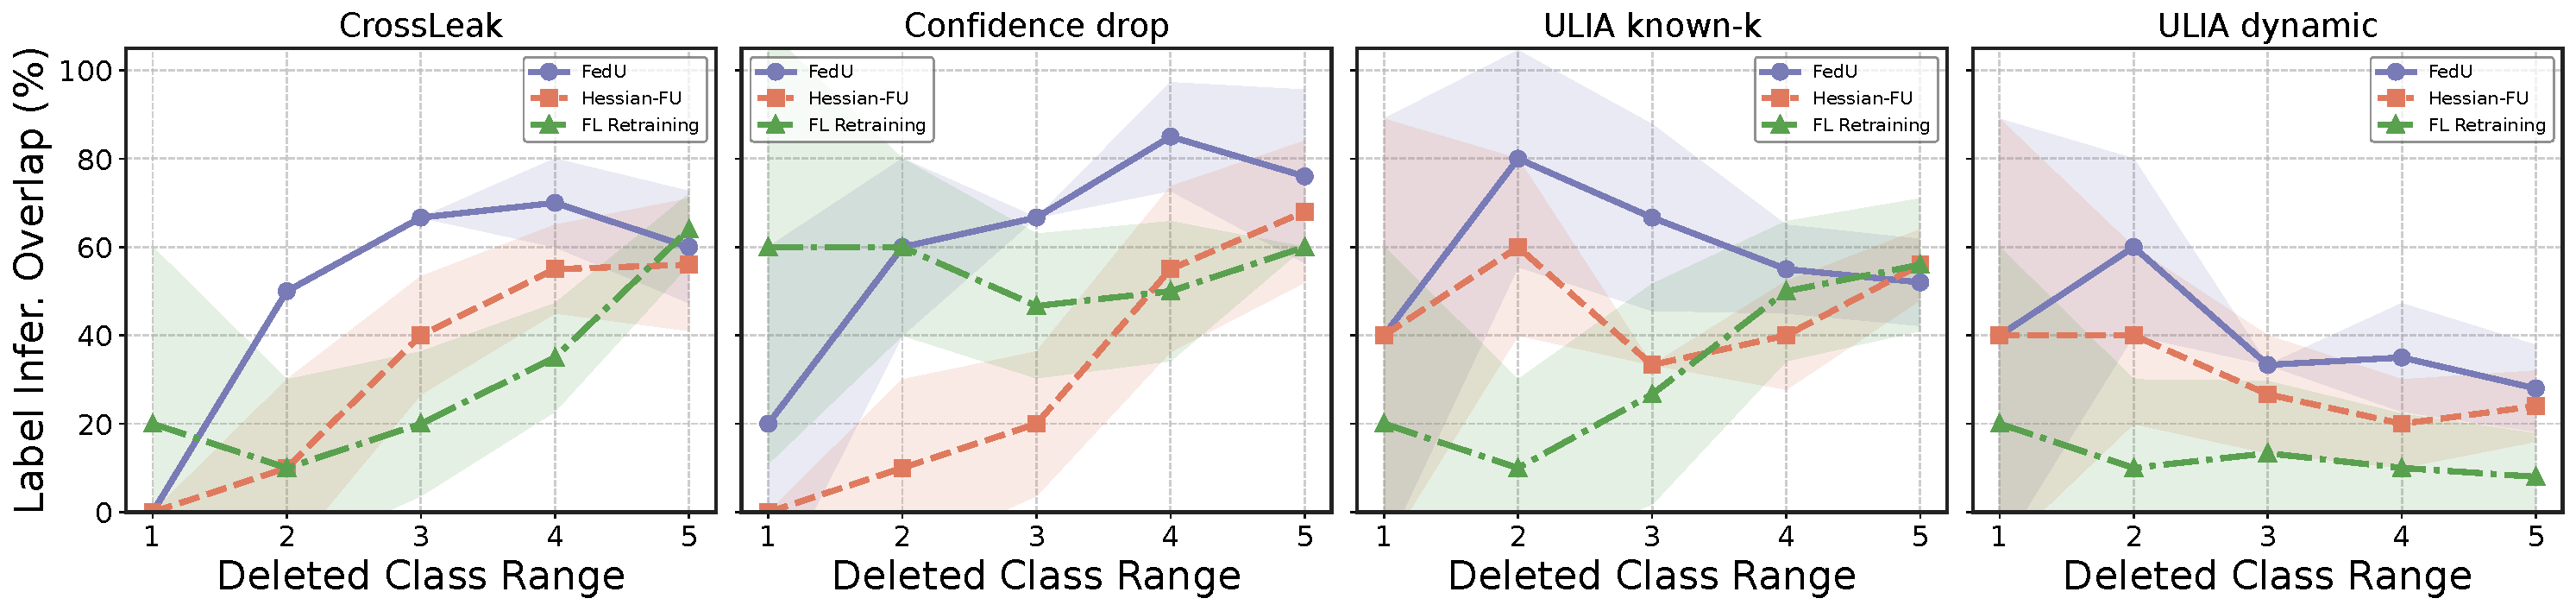
\includegraphics[scale=0.32]{../Exp_results/On_CIFAR10/figures_attacks/CIFAR10_Attacks_label_inference_overlap}
	}
	\caption{Label Inference of Different Deleted Class Ranges}
	\label{fig:label_inf}
\end{figure*}

\begin{figure}[t]
	\centering
	\hspace{-2mm}
	\subfloat{  \rotatebox{90}{ \hspace{3mm}	\footnotesize{On CIFAR10} }
		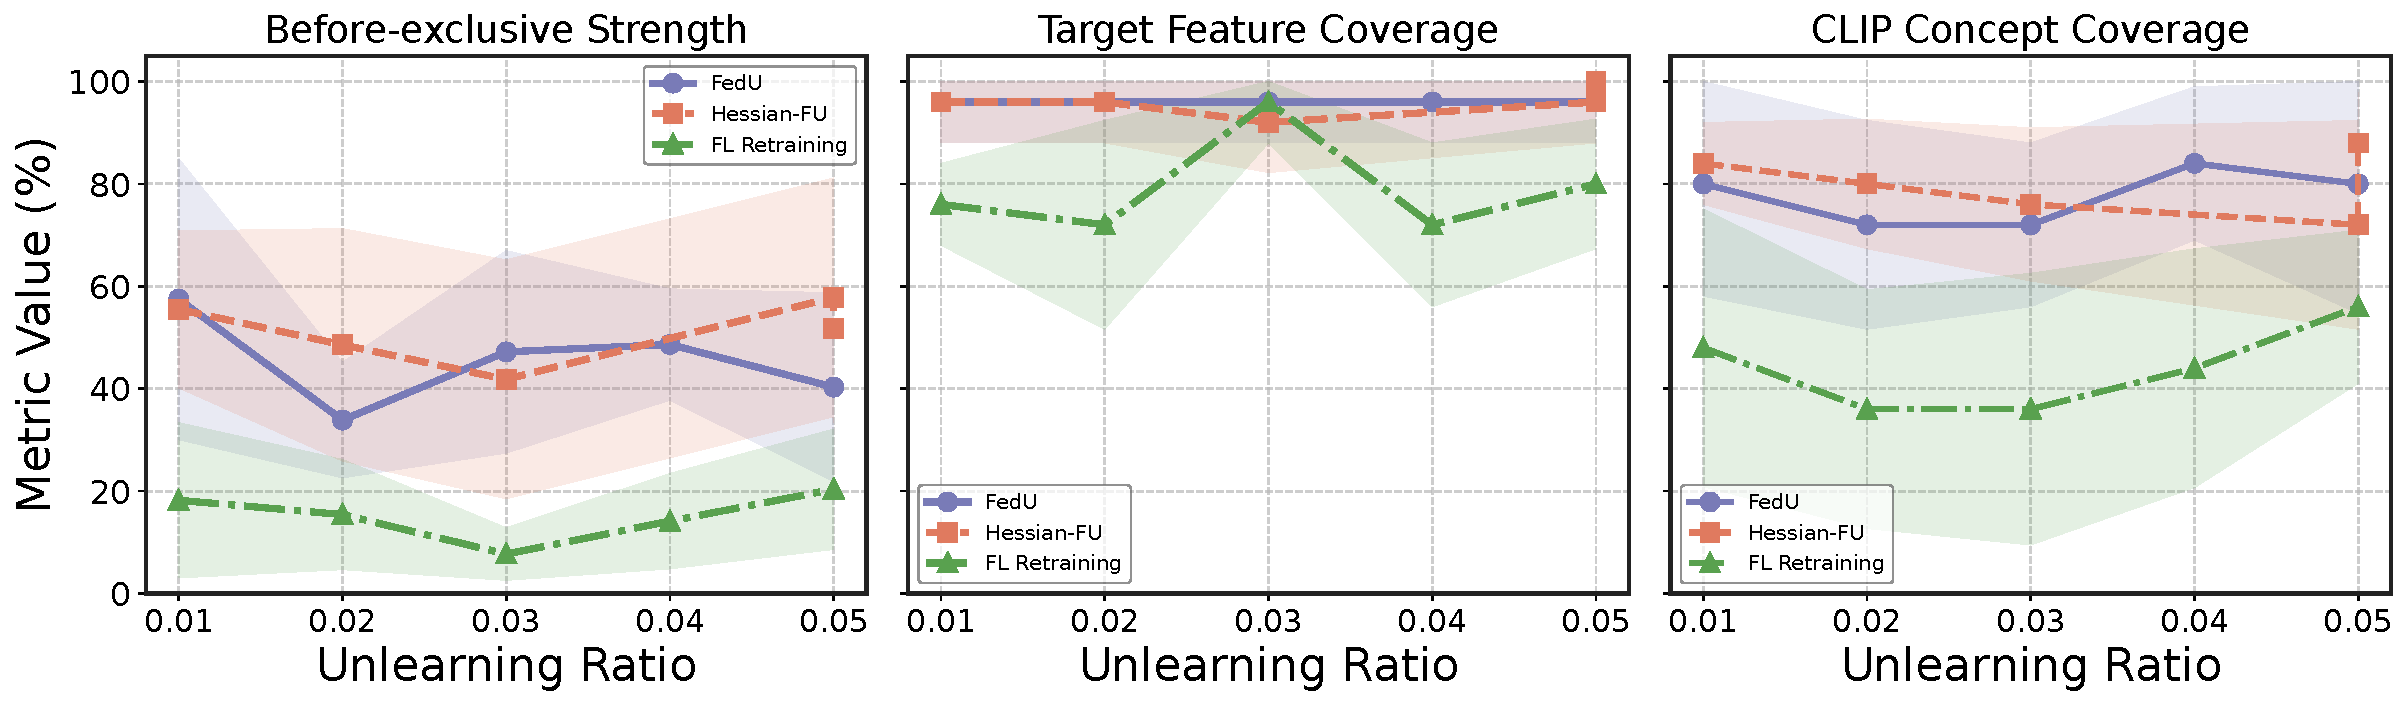
\includegraphics[scale=0.2]{../Exp_results/On_CIFAR10/figures_attacks_ratio/CIFAR10_Attacks_unl_ratio_feature_and_clip}
	}
	\hspace{-2mm}
	\subfloat{  \rotatebox{90}{ \hspace{3mm}	\footnotesize{On CIFAR100} }
		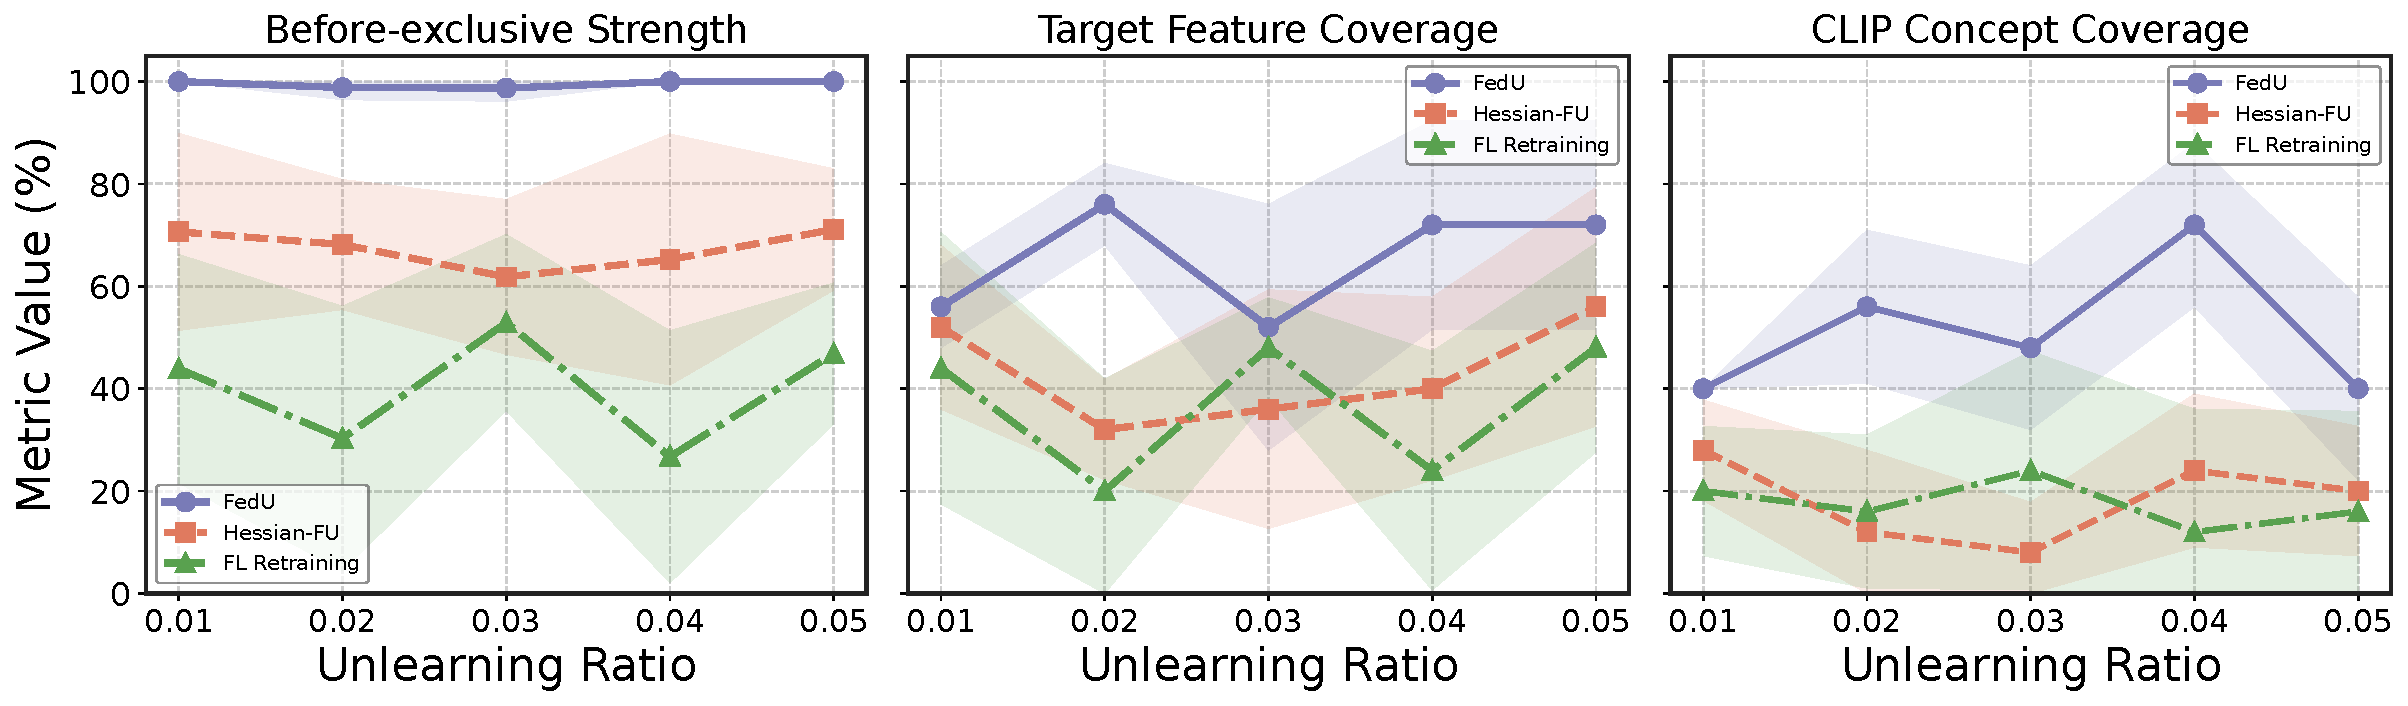
\includegraphics[scale=0.2]{../Exp_results/On_CIFAR100/figures_attacks_ratio/CIFAR100_Attacks_unl_ratio_feature_and_clip}
	}
	\caption{Sensitive Feature Inference of Different Ratio}
	\label{fig:Crossleak_sensitive_feature_inf_ratio}
\end{figure}

\noindent
\textbf{Results.} \Cref{fig:Crossleak_sensitive_feature_inf_ratio} shows that CrossLeak can recover deletion-sensitive evidence beyond deleted labels. On CIFAR10, both FedU and Hessian-FU exhibit high target feature coverage across deletion ratios, indicating that the recovered CrossCoder features are consistently concentrated on the deleted-label region rather than on unrelated retained classes. Their CLIP concept coverage also remains high, showing that the recovered latent features correspond to visually coherent concepts that can be interpreted through top-activating samples. Exact retraining shows weaker before-exclusive strength and lower CLIP coverage, which is expected because retraining removes the deleted samples without applying a localized unlearning update that leaves a strong before-after feature artifact.

On CIFAR100, the leakage pattern is more method-dependent. FedU produces the strongest before-exclusive strength, close to saturation across deletion ratios, which suggests that FedU creates highly separable pre-unlearning feature mass for the removed information. Its target feature coverage and CLIP concept coverage are also higher than those of Hessian-FU and retraining. In contrast, Hessian-FU and retraining still leave measurable feature traces, but their semantic recovery is weaker because CIFAR100 has a larger label space and fewer examples per class, making the top-activating features less visually concentrated. Overall, the results demonstrate that CrossLeak does not only infer which labels were deleted; it can also expose what latent and semantic features were affected by the unlearning request, even without gradients or deleted samples.






\subsection{RQ2: Ablation Study of Different Variables}


\noindent
\textbf{Overall Setup.}
RQ2 studies how the variables influence CrossLeak's leakage signal, making it stronger or weaker. We conducted ablation studies for two key parameters, the \emph{deleted class range} and the number of \emph{unlearning clients}, where the \emph{deleted class range} means the number of target labels included in the unlearning request. We use the same paired-model setting as RQ1, and all curves are averaged over 5 random seeds.




\subsubsection{Influence of Unlearning Range}




\begin{figure}[t]
	\centering
	\hspace{-2mm}
	\subfloat{  \rotatebox{90}{ \hspace{3mm}	\footnotesize{On CIFAR10} }
		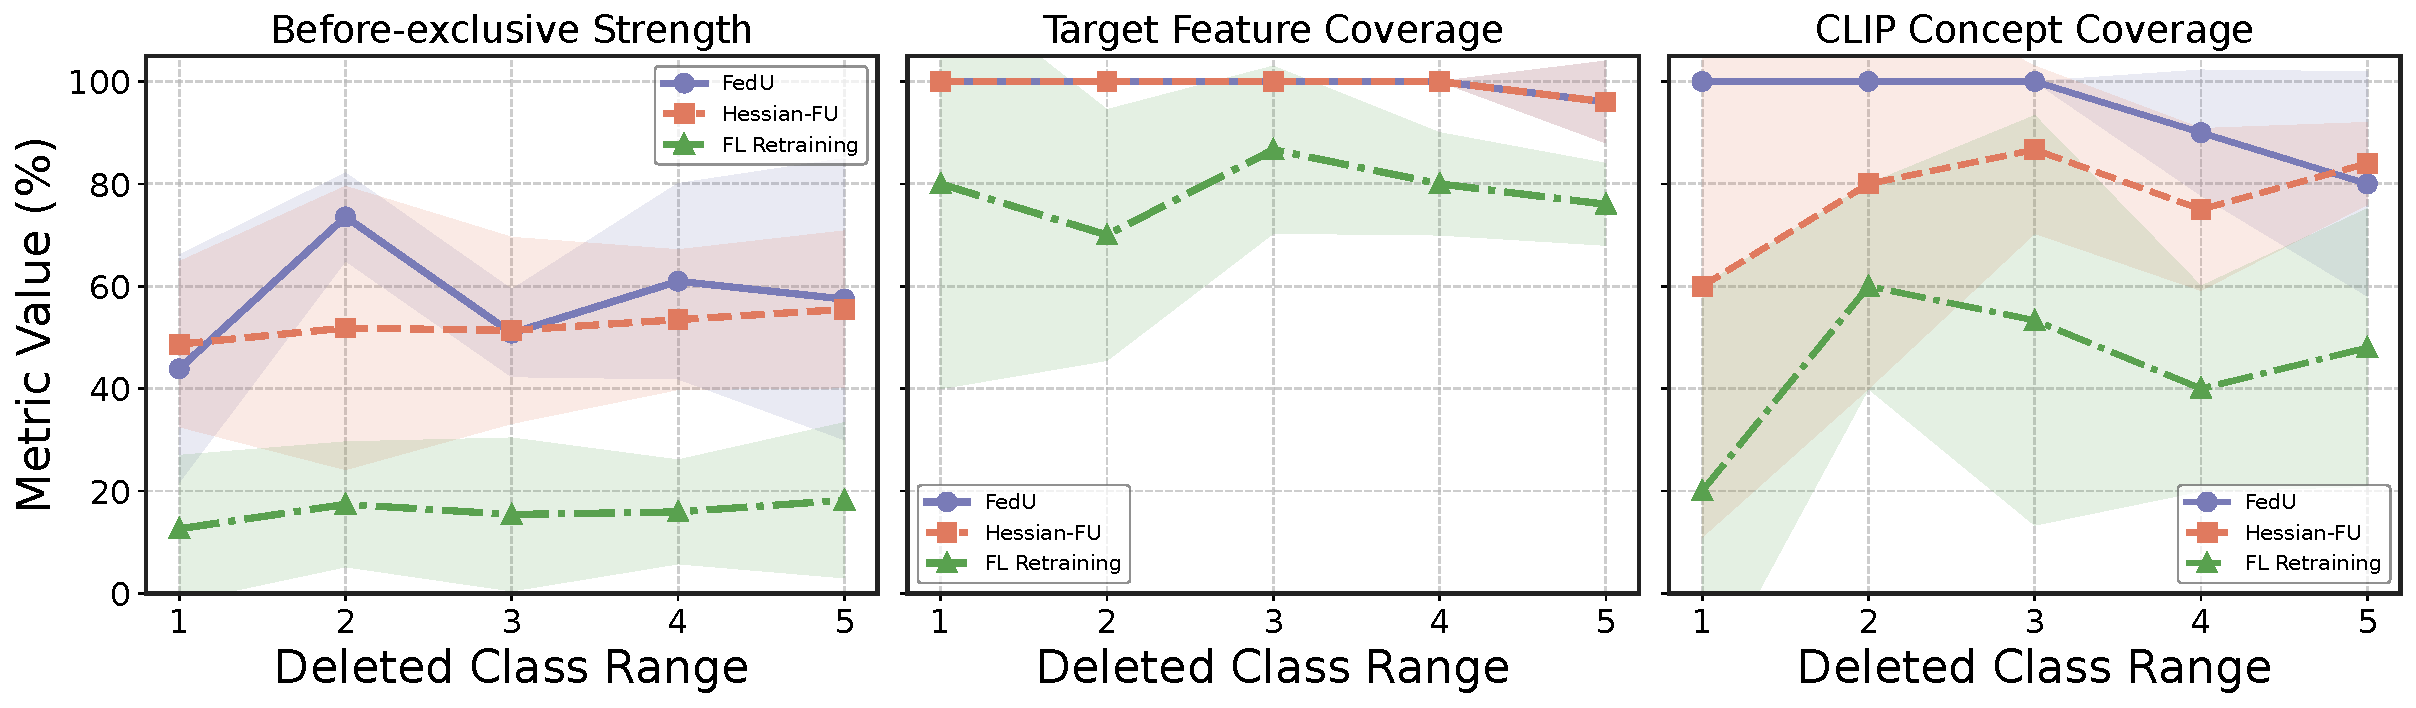
\includegraphics[scale=0.2]{../Exp_results/On_CIFAR10/figures_attacks/CIFAR10_Attacks_feature_and_clip}
	}
	\hspace{-2mm}
	\subfloat{  \rotatebox{90}{ \hspace{3mm}	\footnotesize{On CIFAR100} }
		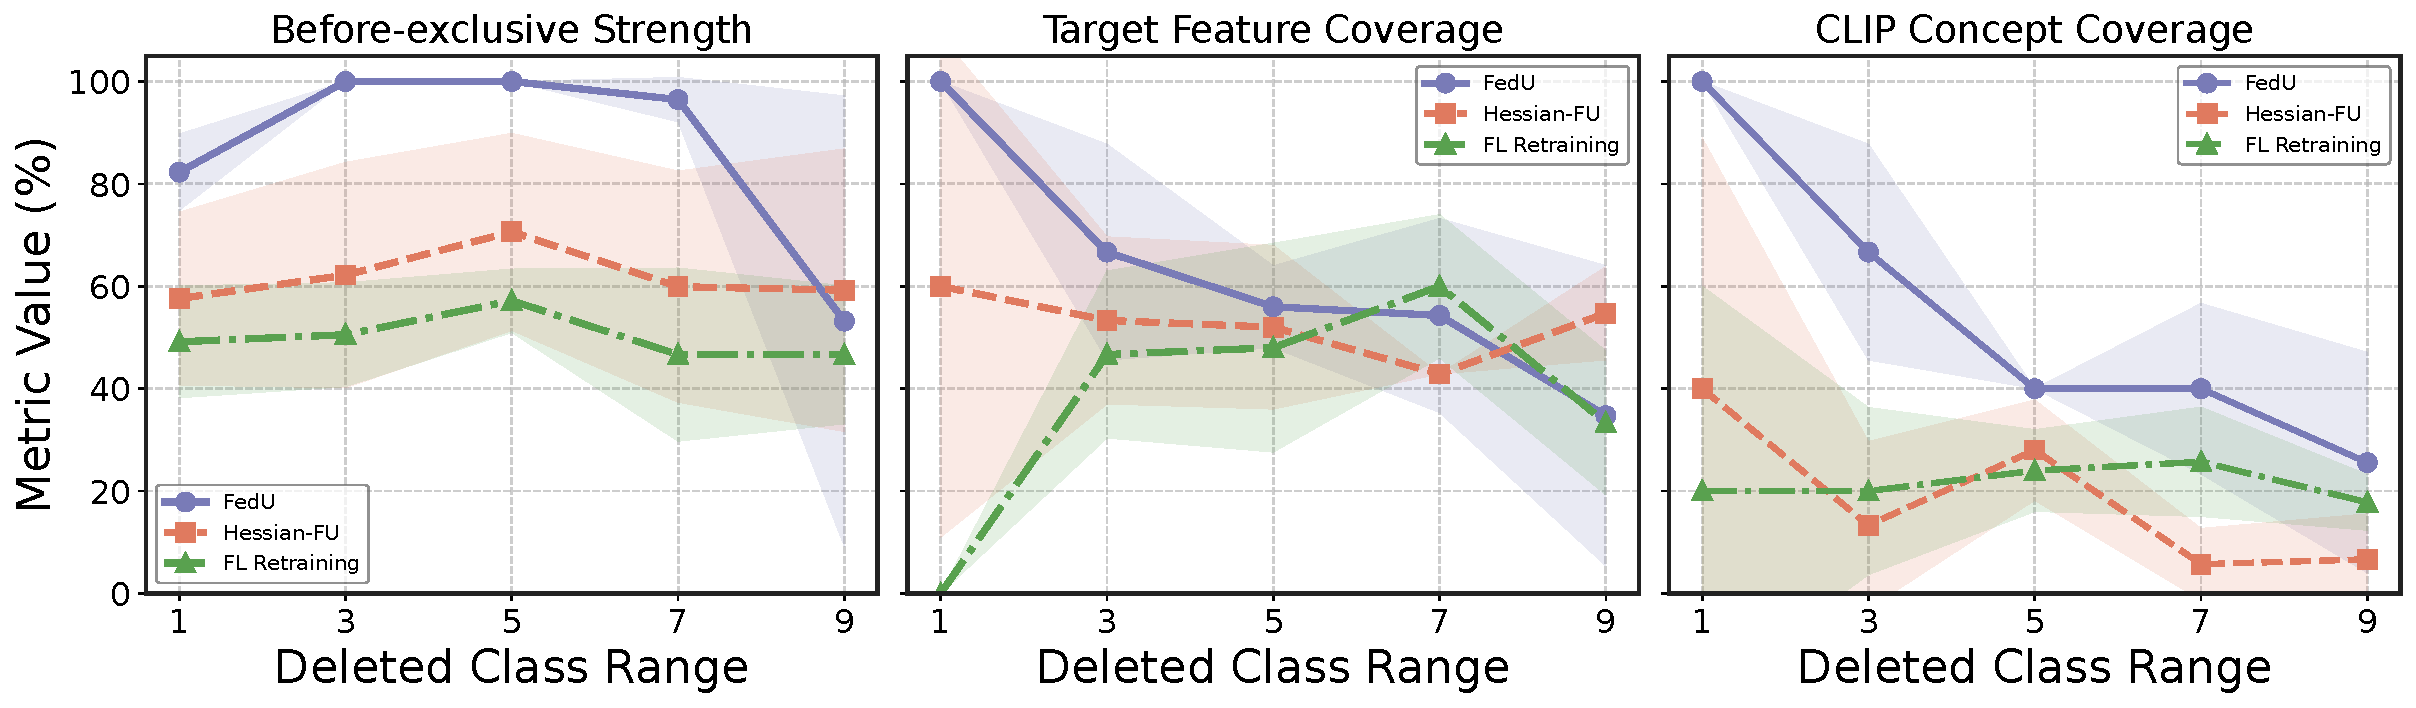
\includegraphics[scale=0.2]{../Exp_results/On_CIFAR100/figures_attacks/CIFAR100_Attacks_feature_and_clip}
	}
	\hspace{-2mm}
\subfloat{  \rotatebox{90}{ \hspace{0mm}	\footnotesize{On TinyImageNet} }
	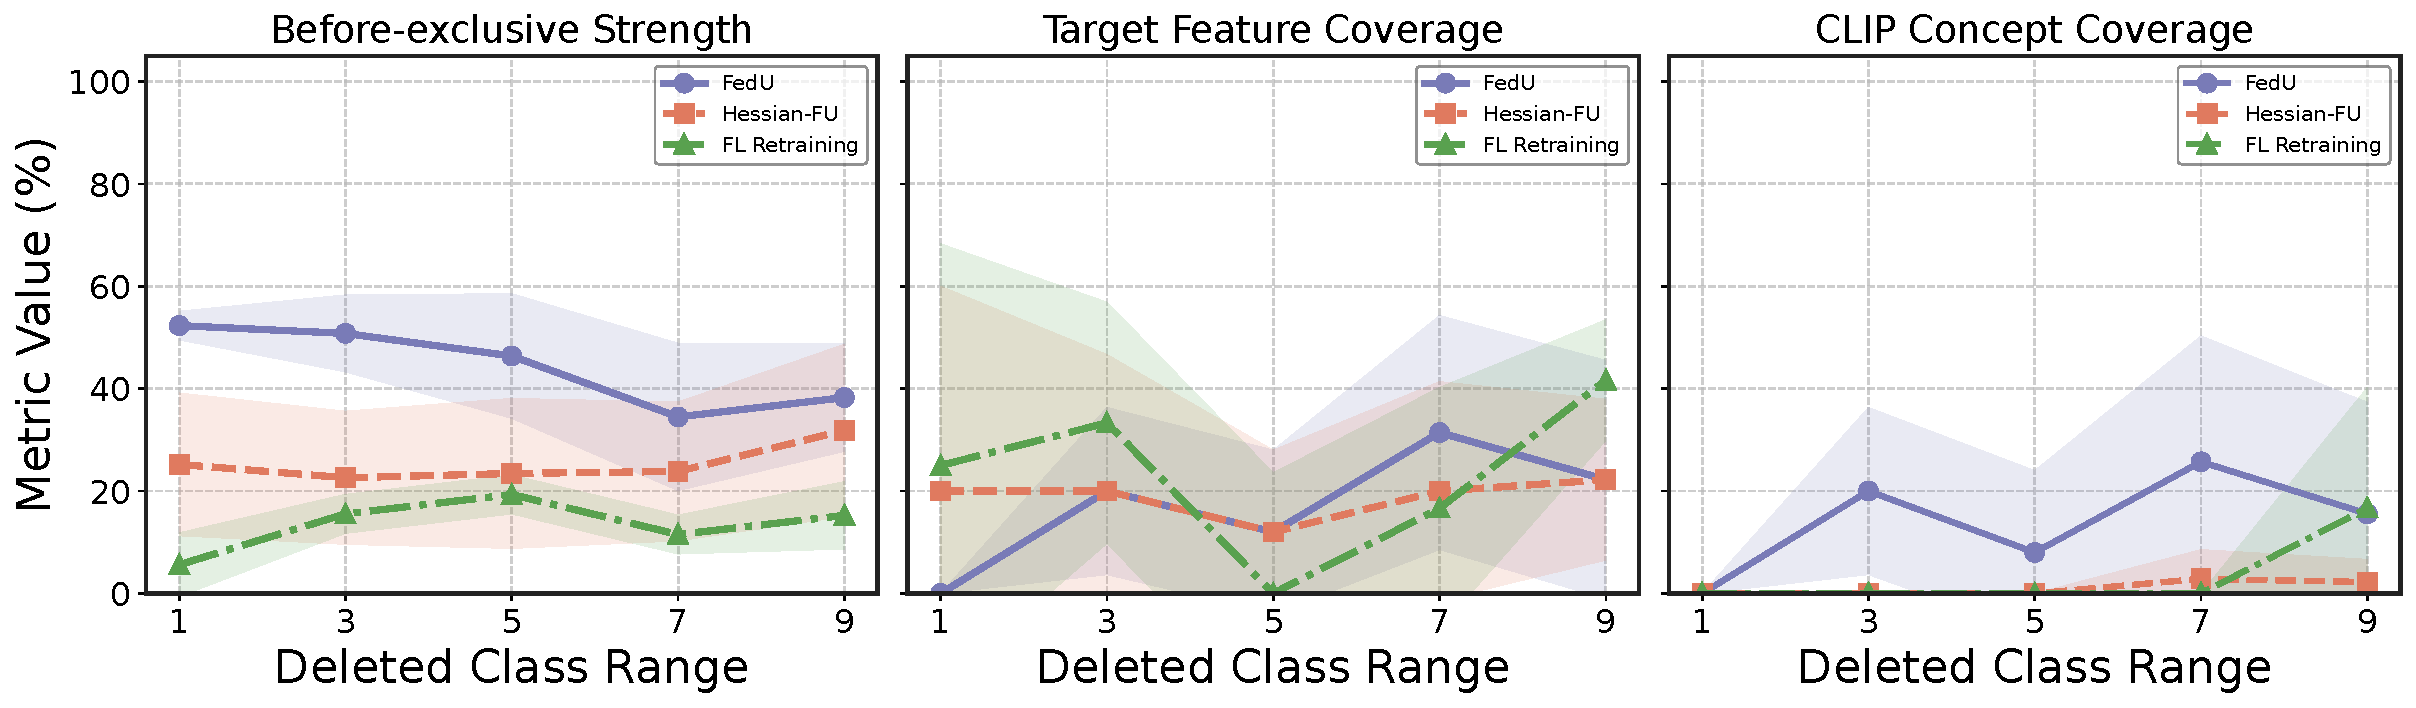
\includegraphics[scale=0.2]{../Exp_results/On_TinyImageNet/figures_attacks/TinyImageNet_Attacks_feature_and_clip}
}
	\caption{Sensitive Feature Inference of Different Deleted Ranges}
	\label{fig:Crossleak_sensitive_feature_inf}
\end{figure}

 

 \begin{figure*}[t]
	\centering
	\hspace{-2mm}
	\subfloat{   	\label{fig:cifar10attacksclientslabelinferenceoverlap}
		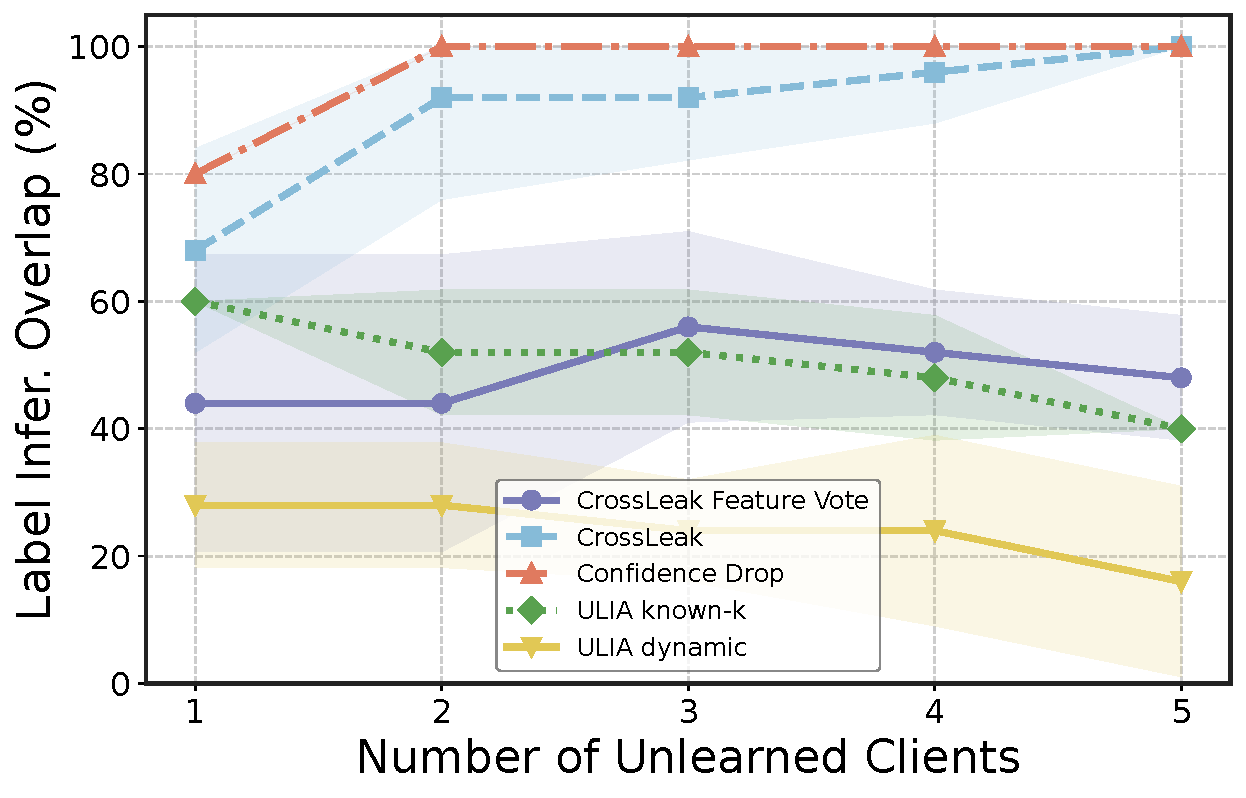
\includegraphics[scale=0.32]{../Exp_results/On_CIFAR10/figures_attacks_clients/CIFAR10_Attacks_clients_label_inference_overlap}
	}
	\hspace{4mm}
	\subfloat{    	\label{fig:cifar10attacksclientsfeatureinferenceperformance}
		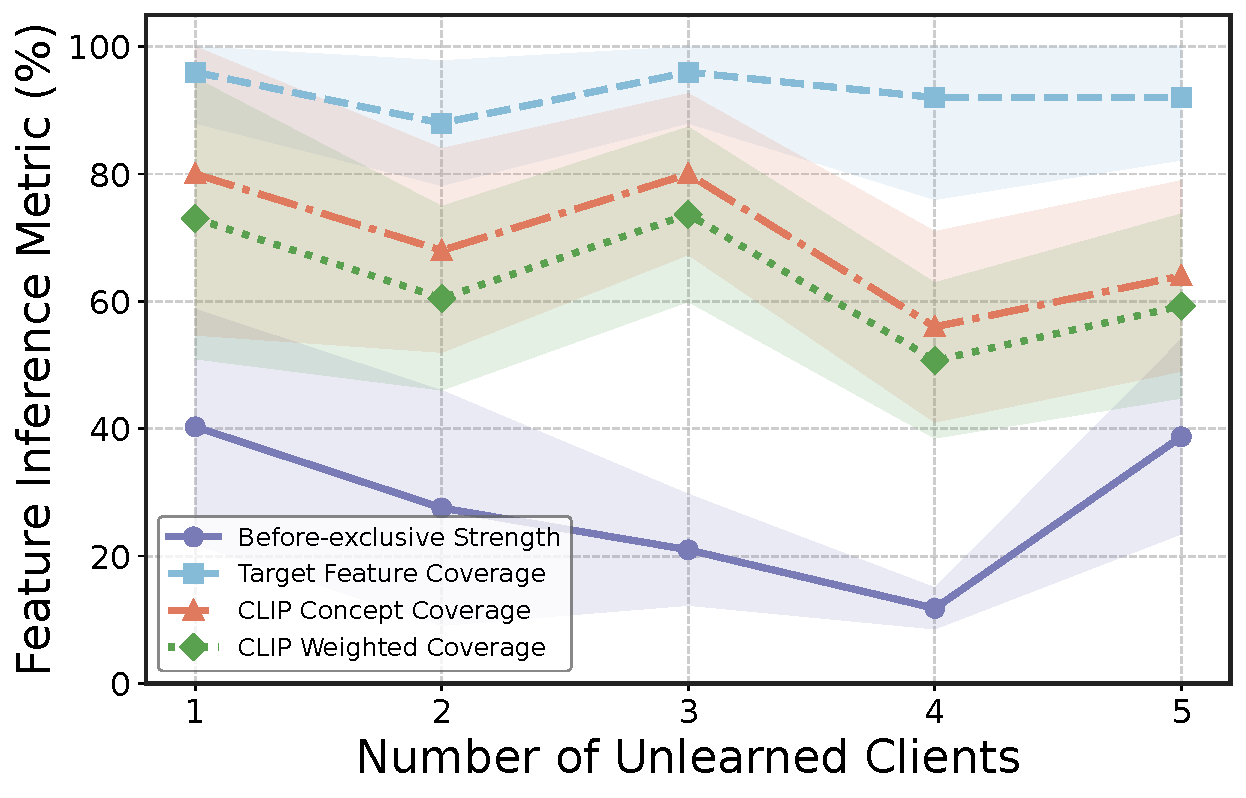
\includegraphics[scale=0.32]{../Exp_results/On_CIFAR10/figures_attacks_clients/CIFAR10_Attacks_clients_feature_inference_performance}
	}
	\caption{CrossLeak on Different Unlearning Clients on CIFAR10}
	\label{fig:Crossleak_cifar10_clients}
\end{figure*}


\Cref{fig:label_inf} shows that the unlearning range has a clear effect on deleted-label inference. On CIFAR10, when the request contains only one deleted class, direct representation and output shifts are weak because a single-class deletion produces a small aggregate change in the model. As the deleted class range increases, the signal becomes more separable: under FedU, confidence drop increases from about $20\%$ overlap at range 1 to about $76\%$ at range 5, while the $\Delta z$ head increases from nearly $0\%$ to about $60\%$. CrossLeak's feature-vote head also improves with the range, reaching about $48\%$ overlap at range 5. This trend indicates that a broader unlearning request leaves a more stable label-level fingerprint across probe samples.

The comparison across inference heads also shows that different heads capture different leakage sources. Confidence drop is the strongest head for FedU because FedU produces visible output-level suppression for deleted labels. ULIA known-k remains competitive when it is given the deletion budget, but ULIA dynamic is less stable as the range grows because threshold-based selection can under-select or over-select labels. Hessian-FU and retraining exhibit weaker label inference at small ranges, yet the confidence-drop and CrossLeak signals become non-trivial at larger ranges. This suggests that even smoother second-order unlearning and retraining can accumulate detectable class-wise shifts when the unlearning request covers more labels. 

\Cref{fig:Crossleak_sensitive_feature_inf} shows that the feature-level leakage is more persistent than label-level overlap. On CIFAR10, CrossLeak maintains high target feature coverage across ranges for FedU and Hessian-FU, with averages close to $99\%$, meaning that the recovered features remain concentrated on the deleted-label region even when the deleted set changes in size. CLIP concept coverage is also high, especially for FedU, showing that the recovered CrossCoder features correspond to semantically meaningful visual concepts rather than only numerical representation artifacts. Exact retraining has much lower before-exclusive strength and weaker CLIP concept coverage, which is consistent with retraining removing deleted data without creating a concentrated unlearning-update artifact.

On CIFAR100 and TinyImageNet, increasing the unlearning range makes semantic recovery harder because the label space is larger and each class contributes fewer examples. FedU still produces strong before-exclusive strength, but target feature coverage and CLIP concept coverage decline as the range grows, indicating that the deletion-sensitive features become more dispersed across fine-grained classes. Hessian-FU and retraining show weaker semantic coverage, although they still leave measurable before-exclusive feature mass. Overall, these results show that CrossLeak benefits from larger unlearning ranges for label inference, while sensitive-feature inference remains informative even when the semantic evidence becomes more diffuse.





\subsubsection{Different Unlearning Clients}





\Cref{fig:Crossleak_cifar10_clients} studies whether CrossLeak remains effective when the unlearning request is distributed over different numbers of clients. The left subfigure shows that deleted-label inference remains strong under multi-client unlearning. Confidence drop and CrossLeak both improve as more clients participate, reaching nearly perfect overlap when the deletion signal is aggregated across multiple clients. In contrast, ULIA dynamic remains much weaker, suggesting that threshold-based label selection is less reliable when the deletion evidence is spread across clients.

The right subfigure further shows that CrossLeak continues to recover deletion-sensitive features. Target feature coverage stays high across client counts, indicating that the recovered CrossCoder features remain concentrated on the deleted-label region. CLIP concept coverage is also consistently non-trivial, which means that many recovered features can still be mapped to semantic concepts. Although the before-exclusive strength varies with the number of unlearning clients, the persistent target and concept coverage show that the paired-model difference still reveals sensitive feature-level evidence.

%Overall, this ablation shows that CrossLeak is not limited to a single-client deletion setting. Multi-client unlearning does not eliminate the leakage; it can even make the deleted-label signal more consistent, while the CrossCoder-based analysis continues to expose deletion-sensitive latent features.





\subsection{RQ3: Generalization and Application}


\noindent
\textbf{Overall Setup.}
To answer RQ3, we consider two complementary scenarios. First, we test CrossLeak across different unlearning algorithms, including FedU, Hessian-FU, and exact federated retraining, on CIFAR10, CIFAR100 and TinyImageNet. The general settings are the same as in RQ1. This experiment asks whether CrossLeak can generalize to different federated unlearning algorithms. 

Second, we evaluate CrossLeak in a backdoor unlearning scenario on CIFAR100. We start from a backdoored federated model with a fixed target label and then issue an unlearning request that removes the backdoored samples from the selected unlearning client. After unlearning, we compare the backdoored model before unlearning and the model after unlearning. The attacker again uses CrossLeak to identify features that are active before unlearning and suppressed after unlearning, trying to infer the backdoor triggers. We use the heatmaps to highlight the suspicious pixels that CrossLeak finds.



\subsubsection{Different Unlearning Methods}


\begin{figure*}[t]
	\centering
	\hspace{-2mm}
	\subfloat[On CIFAR10]{   	\label{fig:cifar10attacksunlratiofeatureoverlapbar}
		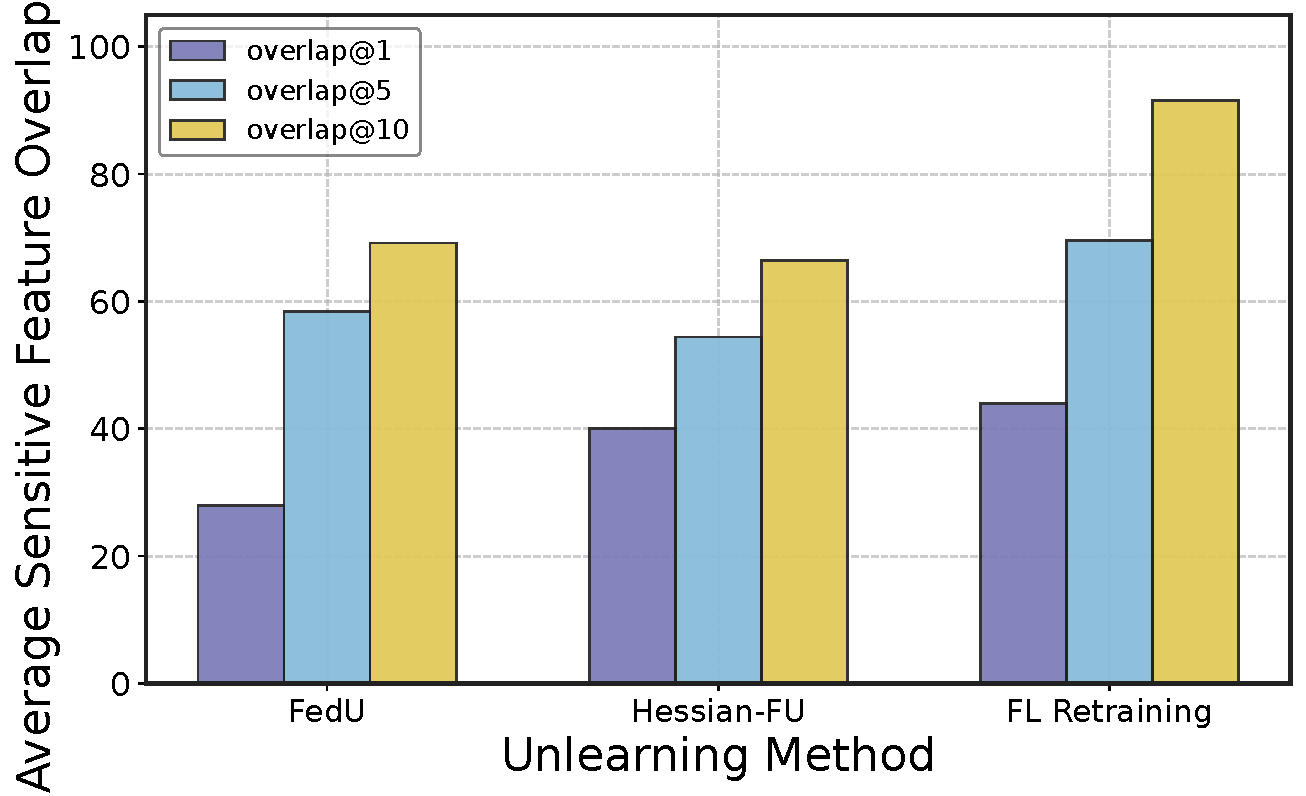
\includegraphics[scale=0.25]{../Exp_results/On_CIFAR10/figures_attacks_ratio/CIFAR10_Attacks_unl_ratio_feature_overlap_bar}
	}
	%	\hspace{-4mm}
	\subfloat[On CIFAR100]{    	\label{fig:cifar100attacksunlratiofeatureoverlapbar}
		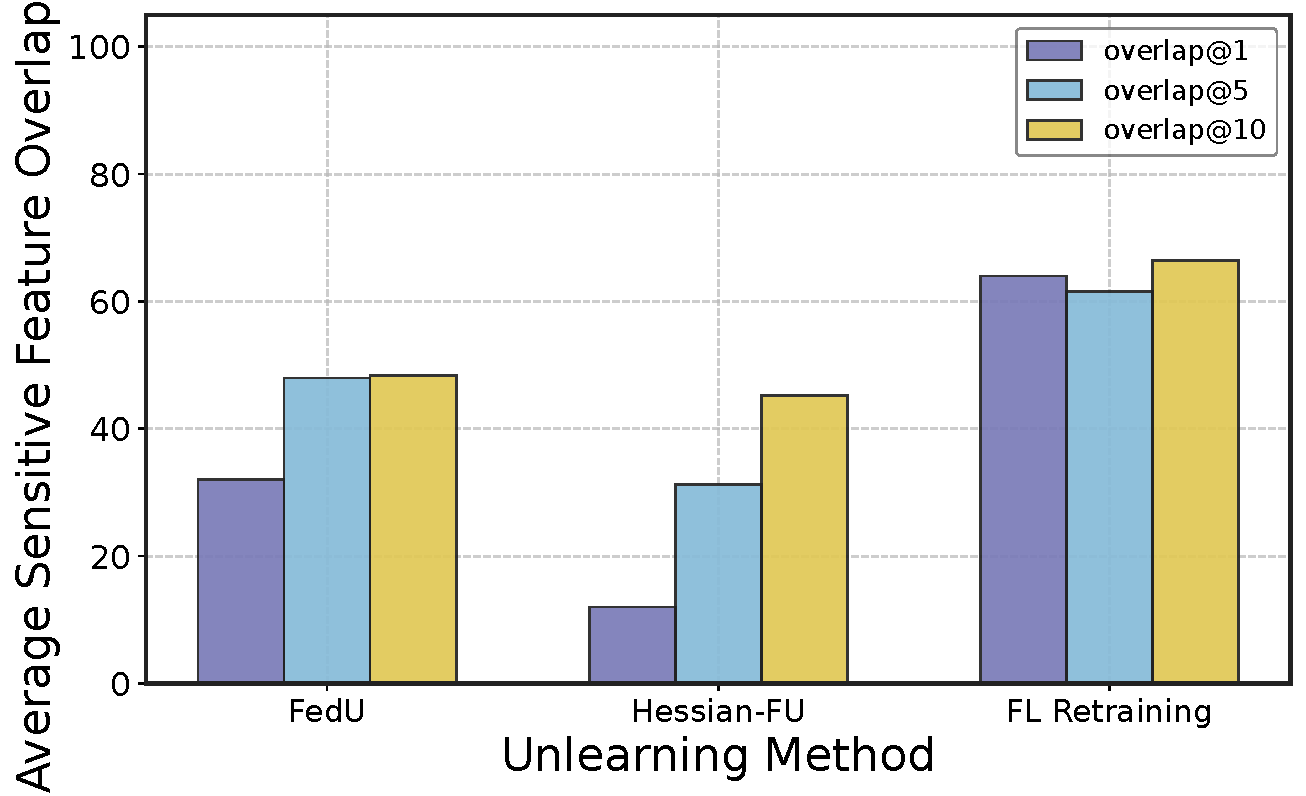
\includegraphics[scale=0.25]{../Exp_results/On_CIFAR100/figures_attacks_ratio/CIFAR100_Attacks_unl_ratio_feature_overlap_bar}
	}
	\subfloat[On TinyImageNet ]{    	\label{fig:tinyimagenetattacksfeatureoverlapbar}
	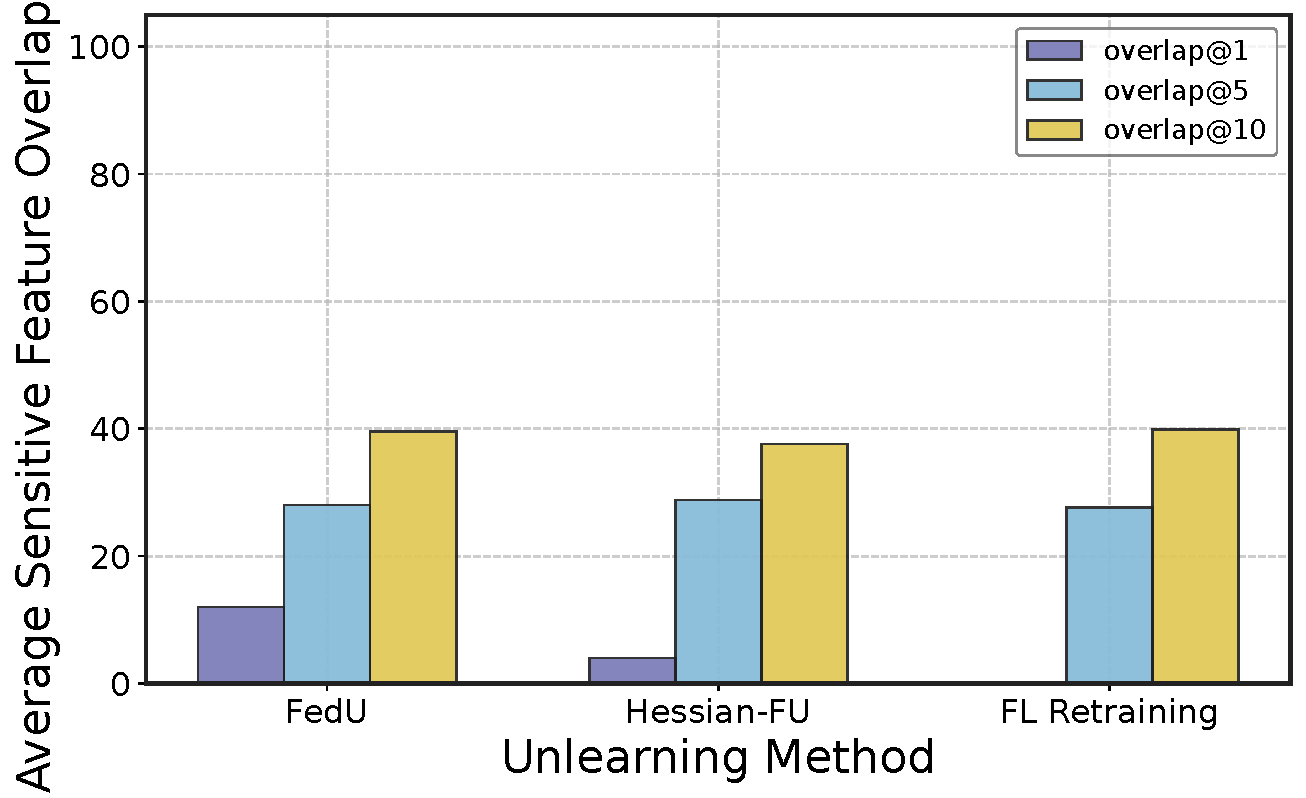
\includegraphics[scale=0.25]{../Exp_results/On_TinyImageNet/figures_attacks/TinyImageNet_Attacks_feature_overlap_bar}
}
	\caption{Sensitive Feature inference by CrossLeak on Different Unlearning Methods}
	\label{fig:Crossleak_of_different_unlearning}
\end{figure*}


 

\Cref{fig:Crossleak_of_different_unlearning} evaluates sensitive feature leakage by comparing feature-overlap@$1$, feature-overlap@$5$, and feature-overlap@$10$ across FedU, Hessian-FU, and exact federated retraining. The three subfigures show a consistent trend: CrossLeak can recover deletion-sensitive features under all evaluated unlearning methods, and the overlap becomes clearer when more top-ranked features are considered.

On CIFAR10, the feature-overlap bars are high for FedU, Hessian-FU, and retraining, and retraining gives the strongest top-$10$ recovery. This means that CrossLeak is not only detecting artifacts from approximate unlearning updates; comparing the original model with an exactly retrained model can also reveal the deleted feature signal. On CIFAR100, the task becomes harder because the label space is larger, but FedU and retraining still show clear feature overlap, while Hessian-FU is weaker in the top-ranked positions. On TinyImageNet, the bars are lower overall, which is expected for a larger and more fine-grained dataset, but the top-$5$ and top-$10$ overlap remains visible for all methods.

%Overall, the figure shows that CrossLeak generalizes across unlearning algorithms and datasets. The leakage is strongest on simpler datasets and weaker on TinyImageNet, but it does not disappear. The gap between top-$1$ and top-$10$ also suggests that unlearning-sensitive evidence is often distributed over several recovered features rather than concentrated in one dominant feature.





\subsubsection{Backdoor Trigger Inference}

\begin{figure}
	\centering
	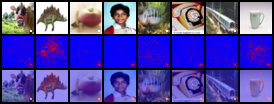
\includegraphics[width=0.97\linewidth]{../On_CIFAR100/backdoored_cifar100/seed_0_backdoor_trigger_heatmap_grid}
	\caption{Backdoor trigger inference on CIFAR100. The heatmaps visualize pixels whose CrossLeak feature scores are strongly associated with the before-unlearning backdoor behavior.}
	\label{fig:seed0backdoortriggerheatmapgrid}
\end{figure}

\Cref{fig:seed0backdoortriggerheatmapgrid} visualizes CrossLeak's trigger-related evidence after backdoor unlearning. Before unlearning, the backdoored model has a high attack success rate on triggered samples, while after unlearning the backdoor accuracy drops close to random behavior. In our multi-seed evaluation, the backdoor accuracy decreases from about $93.0\%$ before unlearning to about $1.5\%$ after unlearning, while the clean accuracy remains almost unchanged. This confirms that the unlearning procedure removes the functional backdoor behavior without simply destroying the clean classifier.

CrossLeak still detects a strong before-exclusive signal on backdoored probe samples. The recovered features have a high before-exclusive fraction, around $96\%$, and a high before-exclusive strength ratio, around $98\%$, showing that the trigger-related evidence is concentrated in features that are active in the backdoored model and suppressed after unlearning. This is the key signal used by CrossLeak to infer that the unlearning request affects a backdoor-related concept rather than only ordinary class information.


The heatmaps in \Cref{fig:seed0backdoortriggerheatmapgrid} provide qualitative evidence for this inference. The highlighted regions often concentrate around visually suspicious or high-response areas of the triggered images, including regions close to the patch location in several examples. Although the heatmaps are not perfectly localized for every image, CrossLeak can reveal that the removed information is associated with a backdoor trigger and can highlight suspicious image regions.


%The heatmaps, \Cref{fig:seed0backdoortriggerheatmapgrid}, provide qualitative evidence for this inference. The highlighted regions often concentrate around visually suspicious or high-response areas of the triggered images, including regions close to the patch location in several examples. However, the heatmaps are not perfectly localized for every image, because the CrossCoder identifies trigger-sensitive representation features rather than being trained as a pixel-level detector. Therefore, we interpret this result as trigger inference rather than exact trigger localization: CrossLeak can reveal that the removed information is associated with a backdoor trigger and can highlight suspicious image regions, but it does not guarantee precise recovery of the trigger mask in every sample.

